\documentclass[12pt, letterpaper]{article}
\usepackage[document]{ragged2e}
\usepackage{graphicx}

\title{CMSC 420 Project 2}
\author{Ryan Crow, Jared Cline, and Joseph Kelly}
\begin{document}
	\begin{center}
	\textbf{Graph Colorability}
	\end{center}
		Graph colorability is the ability to color a graph so that no two same-colored vertices are connected by an edge.
		The graph coloring may be done with \textit{n} \textgreater 1 colors, the most common \textit{n} being 2, 3, and 4.
		2-Colorability can be solved in linear time but all \textit{n}-Colorability problems above \textit{n} \textgreater 2 
		must be solved in polynomial time.
	\begin{center}
	\textbf{Proof of NP Status}
	\end{center}
		The NP status of 3-Colorability can be proved by the time taken to verify a solution that satifies the requirements 
		of a graph with the chromatic number 3. This can be done by taking each edge of the graph, and checking both of the
		attached vertices to make sure they do not have the same color. Because we can represent the maximum number of edges
		with the equation \[ \frac{n(n - 1)}{2} \] the algorithm we implement to check each edge on a graph object will have
		a polynomial runtime of $O(n^2)$. This is due to the following: \(n(n - 1)\) reduces to \(n * n = n^2\), 
		and the denominator of \textit{2} can be ignored in the context of Big O runtime. Therefore, the runtime of an 
		algorithm to verify the 3-Colorability of a graph is polynomial, meaning that 3-Colorability is an NP problem.
	\begin{center}
	\textbf{Proof of NP Hard Status}
	\end{center}
		Throughout this proof I will be using blue to represent true, red to represent false, and purpose to represent NULL.
		To convert 3-SAT to 3-Color we have to create a node for each variable and it's negation.
		Then, we connect each variable to it's negation. This is to ensure that a variable cannot be set to the same value as it's negation.
		\begin{center}
		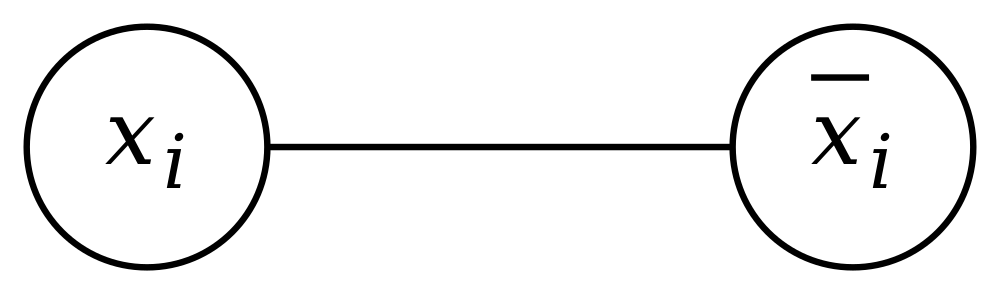
\includegraphics[width=0.5\textwidth]{./var.png}
	\end{center}
		Then we make a triangle and label the nodes: 'N', 'T', and 'F' for null true and false, respectively. Next connect the variable nodes to N.

		\begin{center}
		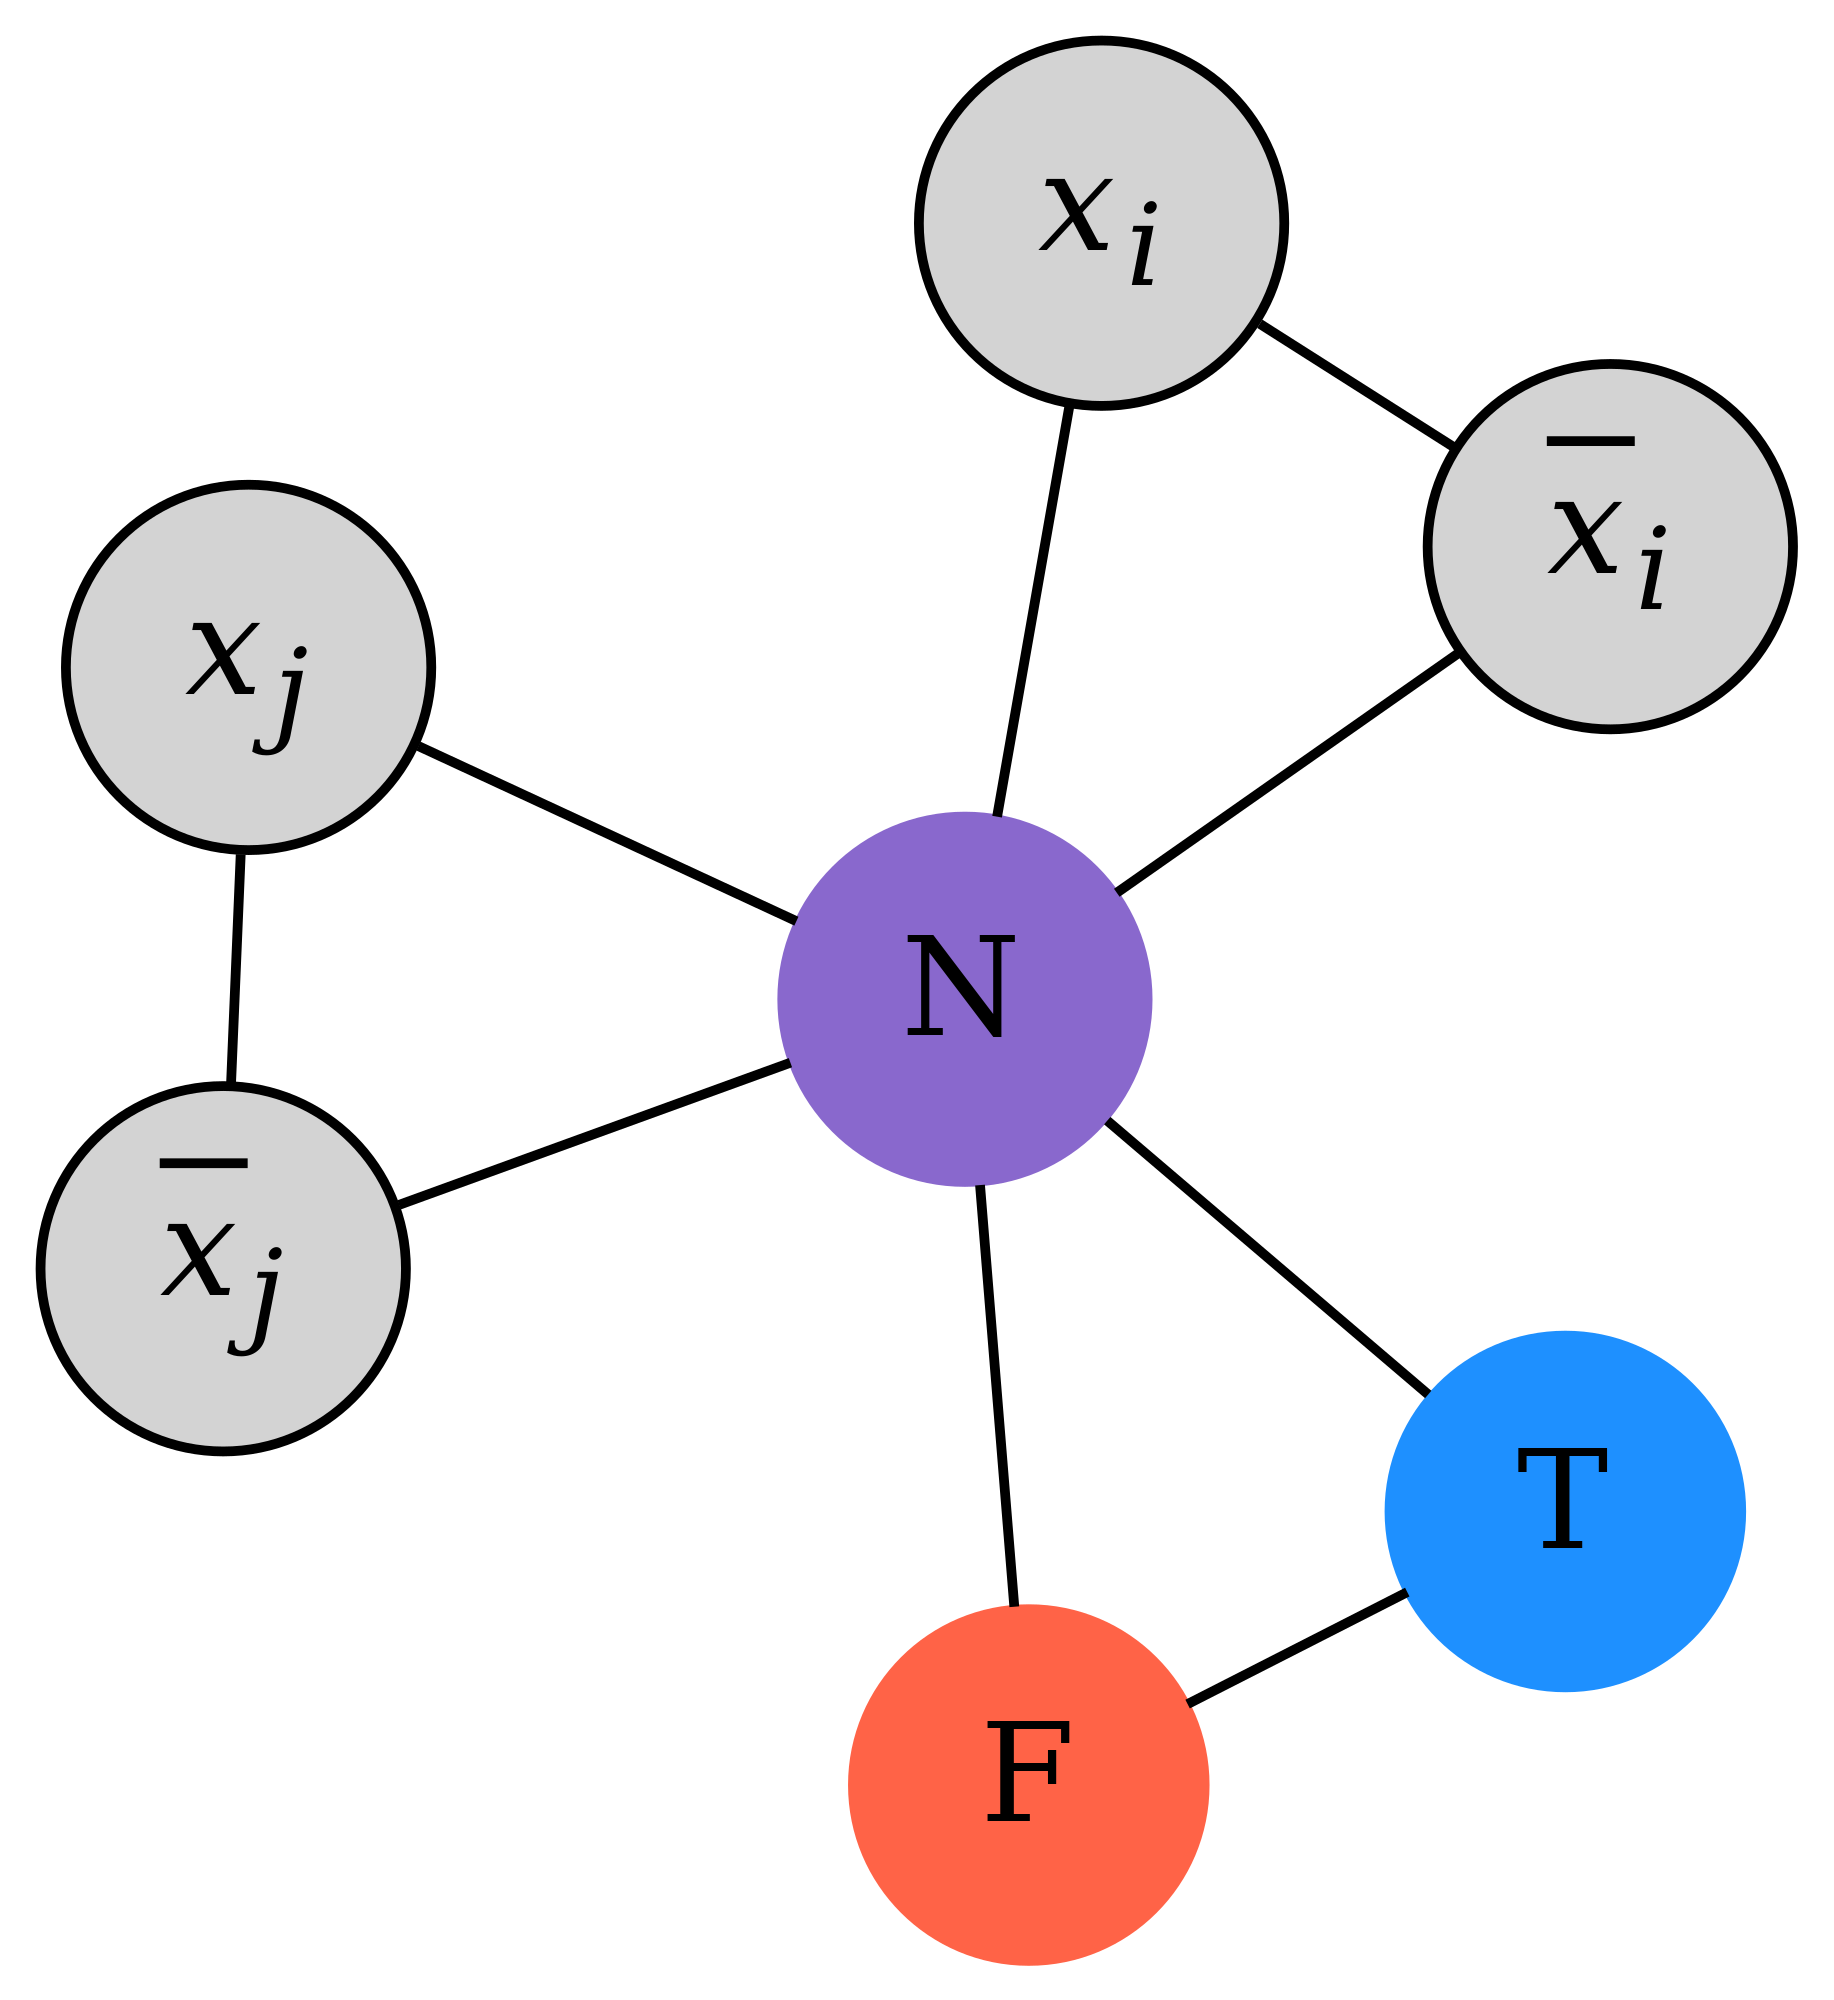
\includegraphics[width=0.5\textwidth]{./triFull.png}
		\end{center}

		For each clause make connect the appropriate variables to a gadget that looks like this:

		\begin{center}
		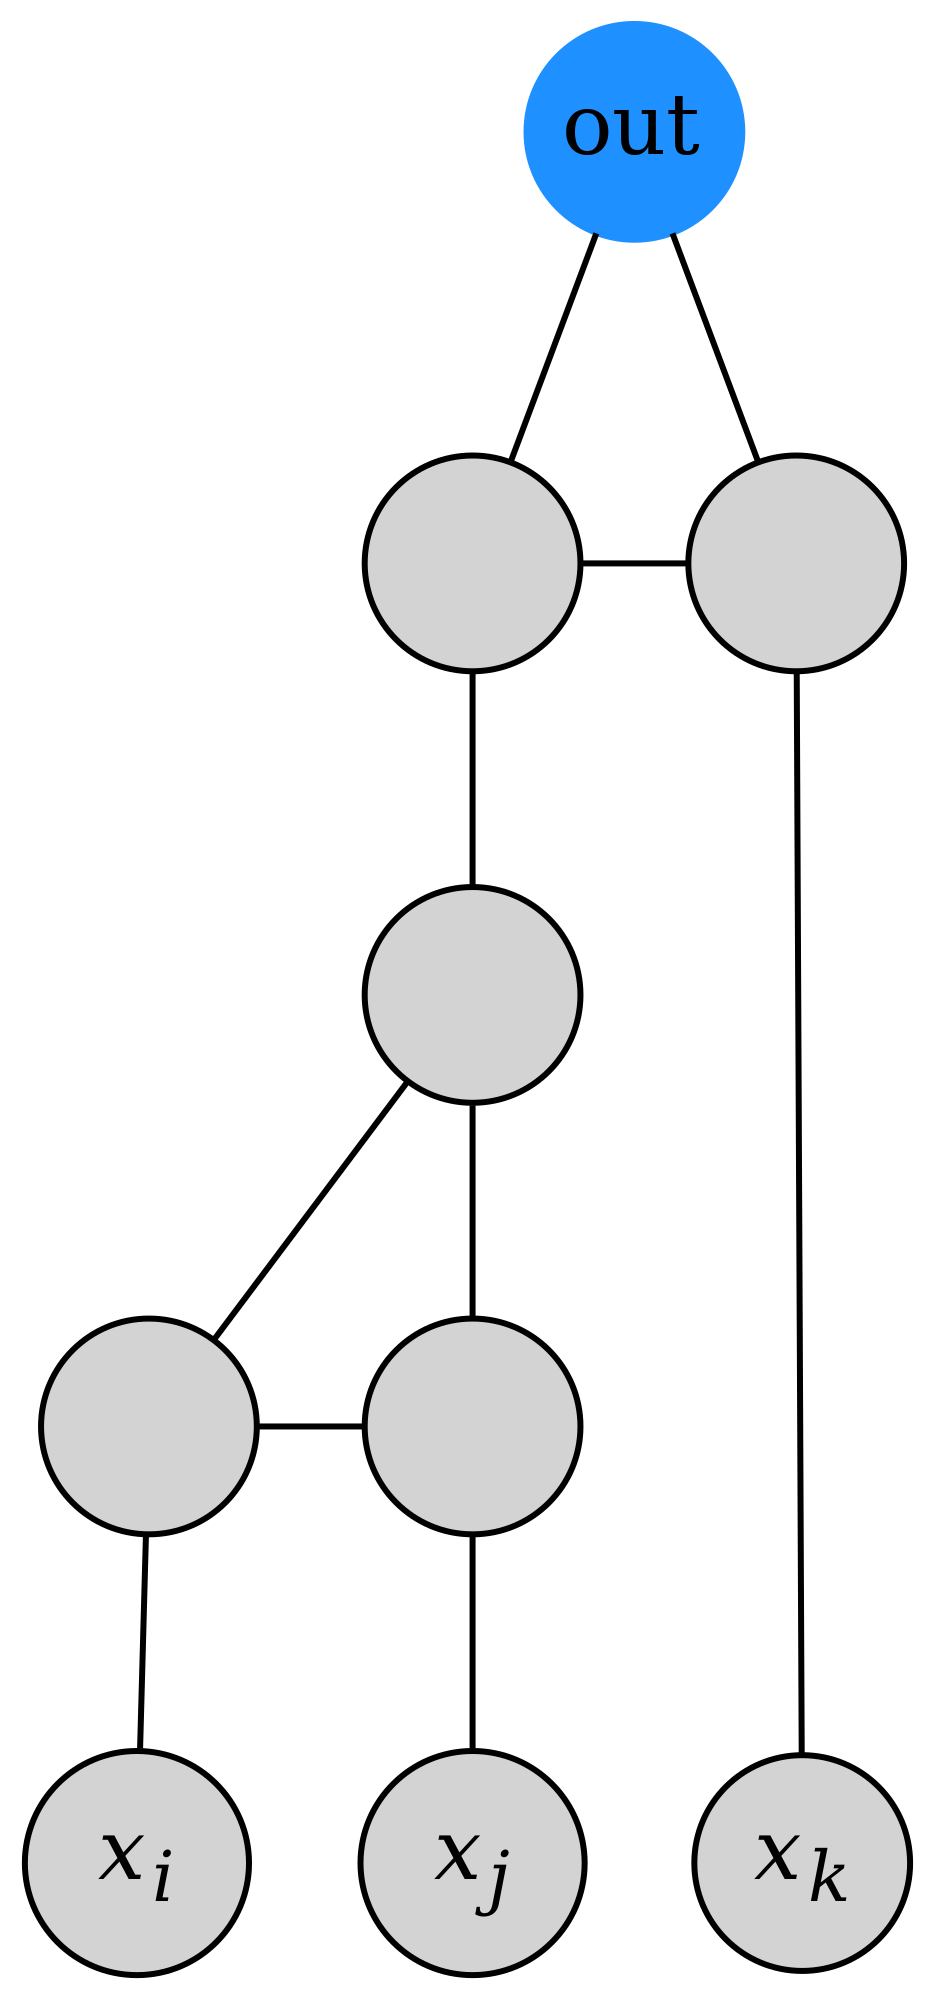
\includegraphics[width=0.25\textwidth]{./clause.png}
		\end{center}

		If all the inputs are colored false the clause won't be colorable to true.

		\begin{center}
		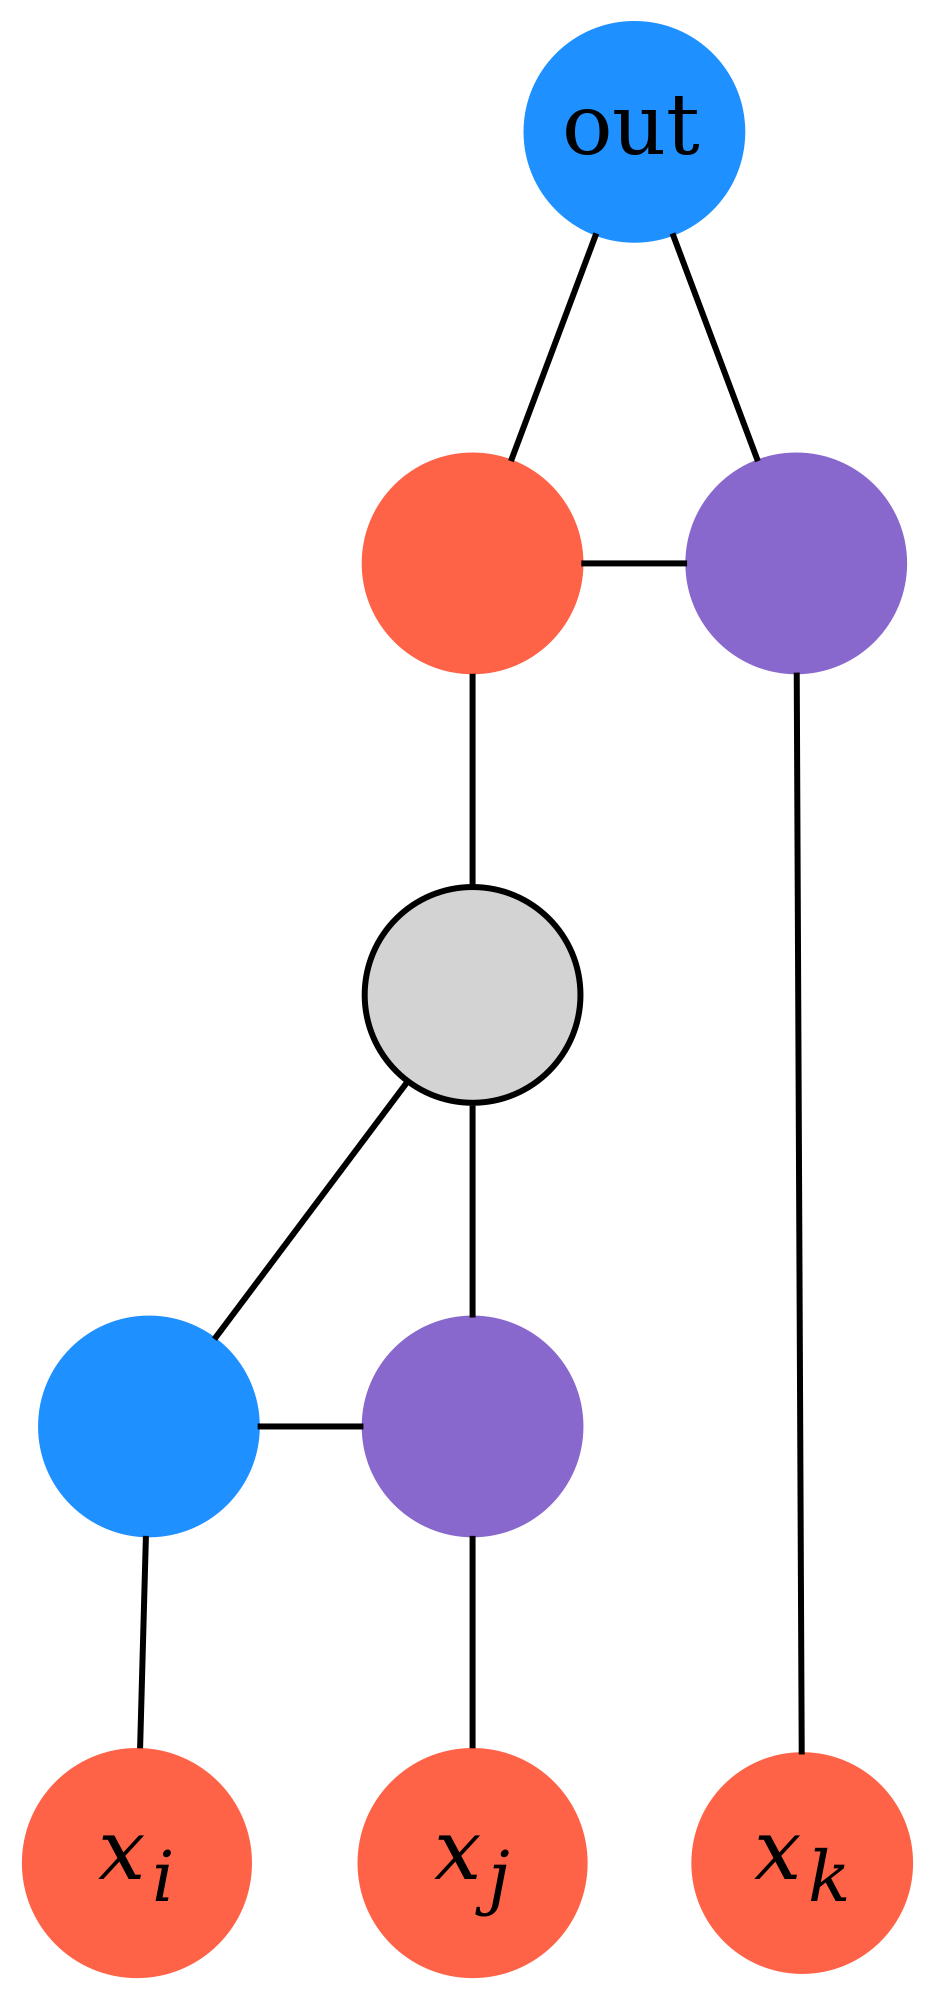
\includegraphics[width=0.25\textwidth]{./clauseProof.png}
		\end{center}

		Finally, connect the output of each to F and N, meaning the output must be colorable to true else the graph isn't 3-colorable.
		If all the variables are colored false, the output can't be colored true. 
		Given the expression $(a|b|c)^(~a|d|e)$ the graph would look like this:

		\begin{center}
		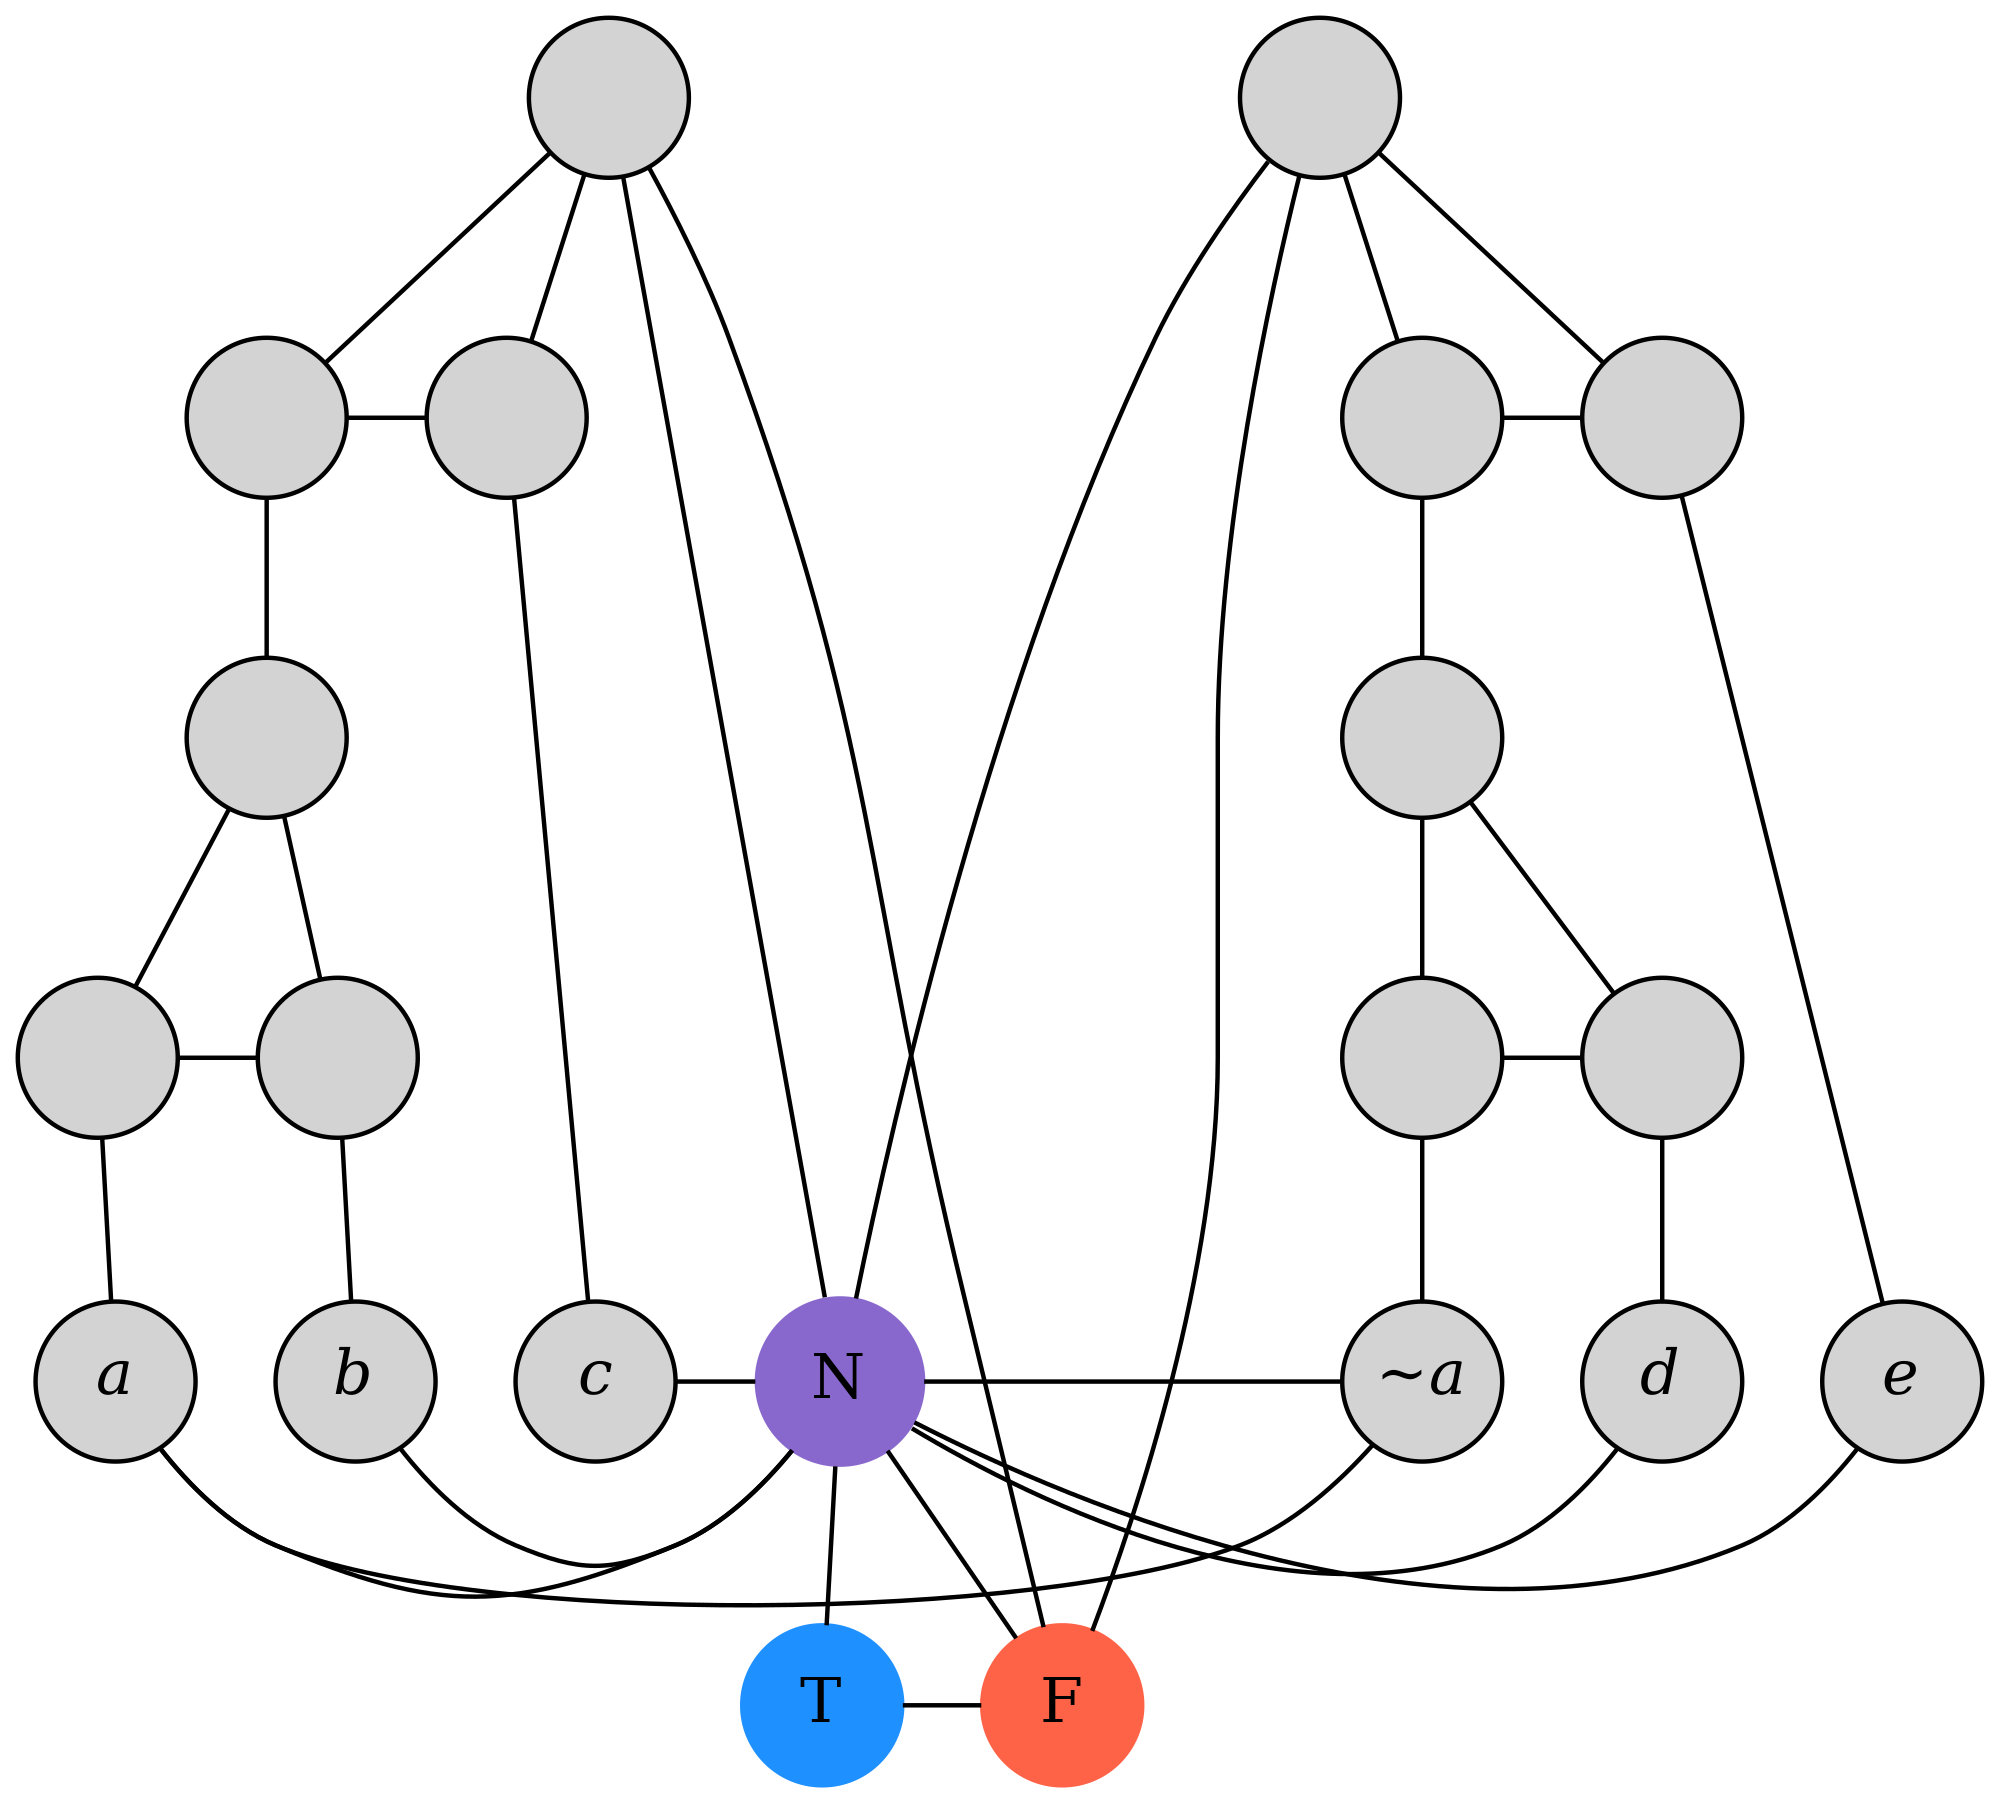
\includegraphics[width=\textwidth]{./gad.png}
		\end{center}

		Since we only add 6 nodes and 12 edges per clause, the size of the gadget doesn't grow exponentially. So we know that the gadget can be constructed in polynomial time.
\end{document}
